\renewcommand{\documentname}{Budget}

\chapter{Budget} \label{section-budget}

This chapter presents the budget for the work. First the internal budget will be calculated taking into account the environment in which we work, and then the budget of the client will be prepared with the necessary items and the benefits applied.

The working time concept is reiterated. Each week has seven working days of three hours each. It is important to bear in mind this concept of working day in order to understand some sections of the budget.

\section{Internal budget}

To calculate the internal budget we must first define our situation. We are two freelancers, a junior and a senior software engineer (see Figure \ref{fig-budget-workers}).


\begin{figure}[H]
    \caption{Freelancers description}
    \label{fig-budget-workers}
  \centering
  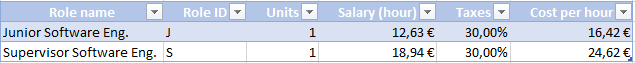
\includegraphics[scale=1]{budget_workers.PNG}
\end{figure}

We have the following rental and amortisation expenses related to the project (see Figure \ref{fig-budget-amortisations}).


\begin{figure}[H]
    \caption{Amortisation costs}
    \label{fig-budget-amortisations}
  \centering
  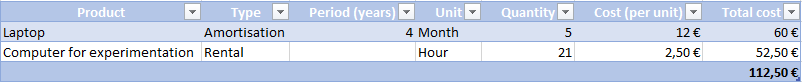
\includegraphics[scale=0.8]{budget_amortisations.PNG}
\end{figure}

Indirect costs are shown below (see Figure \ref{fig-budget-ic}).


\begin{figure}[H]
    \caption{Indirect costs}
    \label{fig-budget-ic}
  \centering
  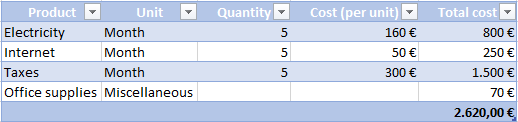
\includegraphics[scale=1]{budget_indirect_costs.PNG}
\end{figure}

Finally, we calculate the costs of carrying out the tasks defined in the WBS.


\begin{figure}[H]
    \caption{WBS Budget costs: Project Management and Analysis}
    \label{fig-budget-wbs-01}
  \centering
  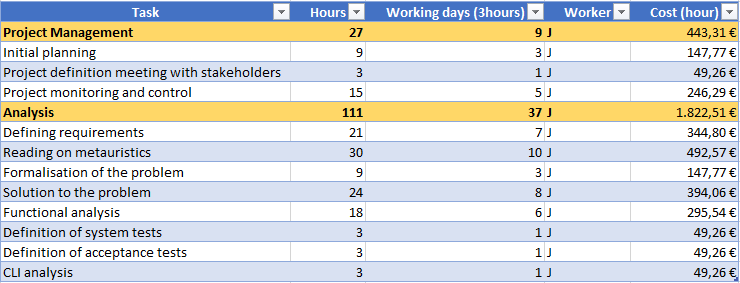
\includegraphics[scale=0.7]{budget_wbs_01.PNG}
\end{figure}


\begin{figure}[H]
    \caption{WBS Budget costs: Design and Development}
    \label{fig-budget-wbs-02}
  \centering
  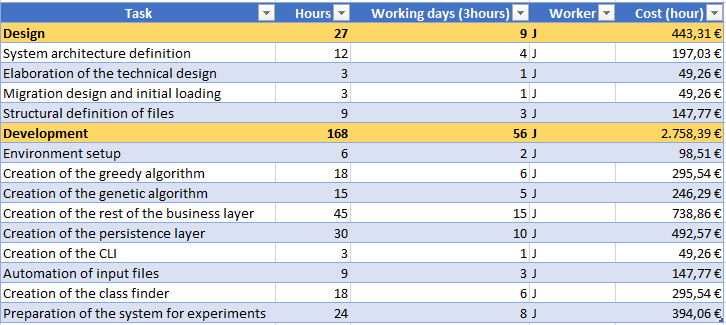
\includegraphics[scale=0.7]{budget_wbs_02.PNG}
\end{figure}


\begin{figure}[H]
    \caption{WBS Budget costs: Documentation, Experiments and Closure}
    \label{fig-budget-wbs-03}
  \centering
  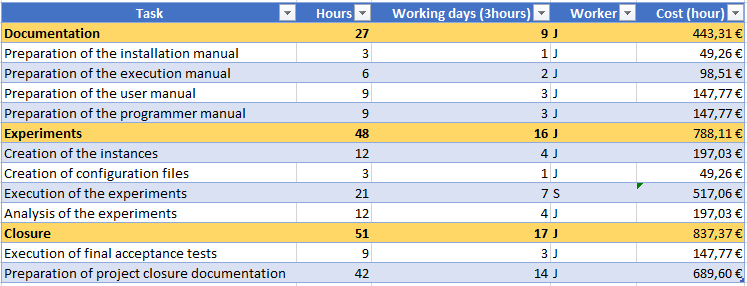
\includegraphics[scale=0.7]{budget_wbs_03.PNG}
\end{figure}

So we are left with the following cost of the WBS phases (see Figure \ref{fig-budget-wbs-sum}).


\begin{figure}[H]
    \caption{WBS Budget costs: Summary}
    \label{fig-budget-wbs-sum}
  \centering
  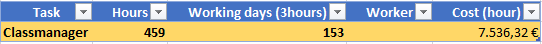
\includegraphics[scale=0.7]{budget_wbs_04.PNG}
\end{figure}

With the addition of all the costs calculated so far, we obtain the internal budget for the project.


\begin{figure}[H]
    \caption{Internal budget}
    \label{fig-budget-internal}
  \centering
  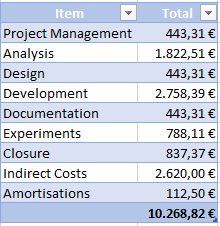
\includegraphics[scale=1]{budget_internal.PNG}
\end{figure}



\section{Client budget}


This project is expected to yield a profit of 25\%. With this information we will proceed to calculate the client's budget. It is important to note that the client will not be shown a budget with all the items, only the generic ones that describe the work to be done. Therefore, we must calculate the amount of the items not shown added to the benefits, and thus obtain a weighting value with which to calculate the client's final budget.

Figure \ref{fig-budget-weight} demonstrates the calculation of this weighting value.


\begin{figure}[H]
    \caption{Weighting value calculation}
    \label{fig-budget-weight}
  \centering
  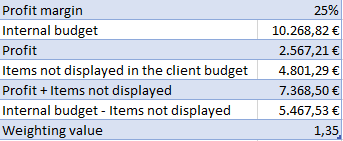
\includegraphics[scale=1]{budget_weighting.PNG}
\end{figure}

Each item is added to its own value multiplied by the weighting value and entered into the client's final budget (See Figure \ref{fig-budget-client}). This means that a cost $c_{i}$ shown in the internal budget will be transformed into a new cost if the item appears in the client budget. This transformation is given by $x_{i} = c_{i} + c_{i} w$, where $w$ is the weighting value. 


\begin{figure}[H]
    \caption{Client budget}
    \label{fig-budget-client}
  \centering
  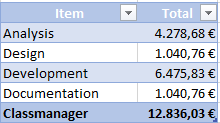
\includegraphics[scale=1]{budget_client.PNG}
\end{figure}




